\chapter{Wstęp}
W dobie przemysłu 4.0 projektowane systemy mają za zadanie nie tylko sterować wybranym procesem, ale także zapewniać jego intuicyjną wizualizację, udostępniać dane innym systemom oraz inteligentnie te dane przetwarzać. Pewnego rodzajem standardem stało się włączenie systemów przemysłowych do internetu. Dzięki takiemu podejściu końcowy użytkownik może z powodzeniem podejrzeć, a nawet wysterować obiekt znajdujący się nawet na drugim końcu świata. Inżynierowie implementujący tak rozbudowane systemu natrafiają na trudności w zintegrowaniu wielu urządzeń pochodzących od różnych producentów, na których zainstalowane są różne systemy operacyjne. Wygodnym rozwiązaniem wydaję się być w takiej sytuacji wykorzystanie technologii webowej, która cieszy się ogromną popularnością.
\newpage
\section{Opis projektu}
W niniejszym projekcie stworzono wielopoziomowy system sterowania linią dozującą napój. Na rysunku \ref{fig:Diagram} przedstawiony został diagram obrazujący ideę działania całego systemu.
\begin{figure}[H]
	\centering
	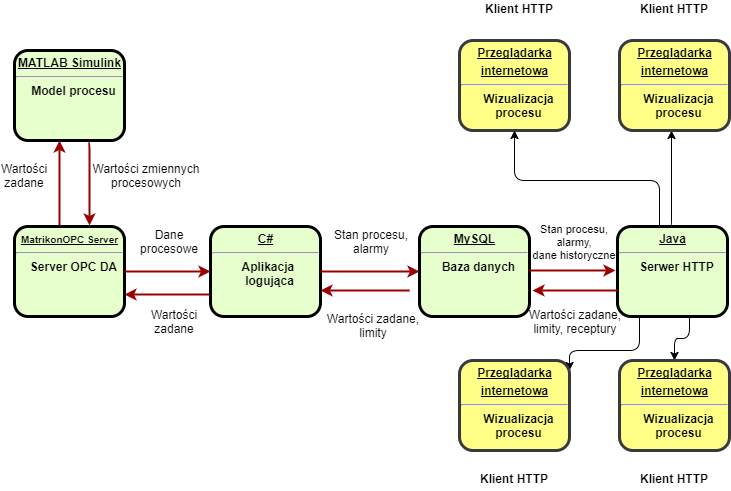
\includegraphics[scale = 0.6]{fig/Diagram.png}
	\caption{Diagram wielopoziomowego systemu sterowania.}
	\label{fig:Diagram}
\end{figure}
Proces mieszania cieczy oraz napełniania butelek zasymulowany został w środowisku MATLAB Simulink. Aktualny stan procesu wysyłany jest na serwer OPC. Dedykowana aplikacja loguje dane z serwera do bazy danych. Serwer HTTP zapewnia klientom wizualizację danych oraz możliwość wysterowania obiektu z poziomu dowolnej przeglądarki internetowej. Każda z wyodrębnionych na rysunku \ref{fig:Diagram} części oprogramowania może pracować niezależnie na różnych komputerach PC, natomiast trudno wyobrazić sobie praktyczny sens takiego rozwiązania. Proponuje się, aby oprogramowanie zaznaczone kolorem zielonym pracowało po stronie serwera, oferując wielu klientom dostęp do wizualizacji bieżącego stanu systemu wraz z systemem alarmowania oraz możliwością wysterowania proces zdalnie, przez internet. 


